% Demonstration of tkz-plot2d
% Author: Alain Matthes
% Note: Requires GNUPLOT
\documentclass{article}
\usepackage[usenames,dvipsnames]{xcolor}
\usepackage{tikz,tkz-plot2d,amsmath}
\usetikzlibrary{arrows}%
\usepackage[np,autolanguage]{numprint}
\usepackage{verbatim}

\begin{comment}
:Title: tkz-plot2d
:Tags: Plots, GNUPLOT

A collection of plots created with the TikZ-based `tkz-plot2d`_ package.
Provides among other things, convenient macros for creating axes and grids.

Requires GNUPLOT_. Documentation_ only available in French.

:Author: Alain Matthes
:Source: `Altermundus.fr`_

.. _documentation: http://www.altermundus.fr/pages/downloads/doc-TKZplot2d.pdf
.. _tkz-plot2d: http://www.altermundus.fr/pages/pdflatex/plot2d.html
.. _Altermundus.fr: http://altermundus.fr/pages/lx/tk.html
.. _GNUPLOT: http://www.fauskes.net/pgftikzexamples/gnuplot-basics/


\end{comment}

\begin{document}
\begin{preview}

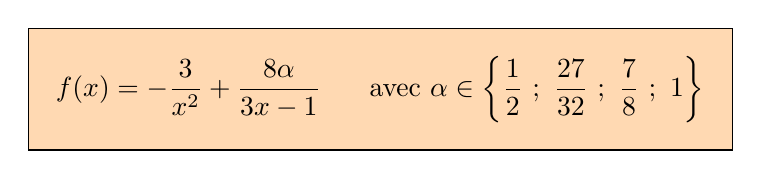
\begin{tikzpicture}[xscale=4,yscale=1]
    \tkzinit[xmax=3,ymax=3,ymin=-4];
    \tkzgrid
    \tkzx
    \tkzy
    \tkzfct[color=red](0.35..3){-3/(x*x) +4/(3*x-1)}
    \tkzfct[color=blue](0.35..3){-3/(x*x) +27/(4*(3*x-1))}
    \tkzfct[color=orange](0.35..3){-3/(x*x) +8/(3*x-1)}
    \tkzfct[color=green](0.35..3){-3/(x*x) +7/(3*x-1)}
    \node[draw,inner sep =10pt,fill=orange!30] at (2,-2)%
        {$f(x)=-\dfrac{3}{x^2}+\dfrac{8\alpha}{3x-1}$%
    \hspace{.5cm} avec%
    \ $\alpha \in%
    \left\{\dfrac{1}{2}~;~\dfrac{27}{32}~;~\dfrac{7}{8}~;~1\right\}$};
\end{tikzpicture}%
%
\begin{tikzpicture}[scale=1]
    \tkzinit[xmin=-2,xmax=3,ymax=3]
    \tkzgrid[color=orange](-2,0)(3,3)
    \tkzx[orig]
    \tkzy
    \tkzfct[label = false,%
    samples = 200,%
    lw = 1pt,
    color = red](-1..2)%
    {(x*x*x+x*x)**(0.5)}
    \tkztg{\tkzfcta}(0)
    \tkztxt[style = {draw},%
    color = red,%
    bkgcolor = orange!20](2,1)%
    {$f(x)=\sqrt{x^3+x^2}$}
\end{tikzpicture}\\%
%
%
\begin{tikzpicture}[scale=1.4]%
    \tkzinit[xmax=800,xstep=100,ymax=2000,ystep=400]
    \tkzgrid[xstep=100,ystep=400](0,0)(800,2000)
    \tkzx
    \tkzy
    \tkzfct[lw=0.8pt](0..800)%
        {(1./90000)*\x*\x*\x-(1./100)*\x*\x+(113./36)*\x}
    \tkzpt[coord](450,400){A}
    \tkzpt(800,1800){}
    \tkztg[color=blue,lw=.8pt,kr=300,kl=450]{\tkzfcta}(450)
    \tkztxt[style    = draw,%
            color    = black,%
            bkgcolor = bistre!50]%
        (300,1200)%
    {$f(x)=\dfrac{1}{90000}x^3 -\dfrac{1}{{100}}x^2 +\dfrac{113}{36}x$}
\end{tikzpicture}%
%
\begin{tikzpicture}%
    \tkzinit[xmax=6,ymax=7]
    \tkzgrid(0,0)(6,7)
    \tkzx
    \tkzy
    \tkzfct[label=false](0..6){x}
    \tkzfct[label=false](6..-0.5){log(x)}
    \tkzairefg[color=orange!60](1..5){\tkzfctgnua}{\tkzfctgnub}
    \rep%
\end{tikzpicture}%
\end{preview}
\end{document}
